\documentclass[12pt]{article}
\usepackage[utf8]{inputenc}
\usepackage{graphicx} % Allows you to insert figures
\usepackage{amsmath} % Allows you to do equations
\usepackage{fancyhdr} % Formats the header
\usepackage{geometry} % Formats the paper size, orientation, and margins
\usepackage[style=authoryear-ibid,backend=biber]{biblatex} % Allows you to do citations - does Harvard style and compatible with Zotero
\addbibresource{Example.bib} % Tells LaTeX where the citations are coming from. This is imported from Zotero
\usepackage[english]{babel}
\usepackage{csquotes}
\usepackage{background}
\usepackage{minted}
\renewcommand*{\nameyeardelim}{\addcomma\space} % Adds comma in in-text citations
\linespread{1.5} % About 1.5 spacing in Word
\setlength{\parindent}{0pt} % No paragraph indents
\setlength{\parskip}{1em} % Paragraphs separated by one line
\renewcommand{\headrulewidth}{0pt} % Removes line in header
\geometry{a4paper, portrait, margin=1in}
\setlength{\headheight}{14.49998pt}
\backgroundsetup{scale=1,angle=0,opacity=0.175,contents={
\includegraphics[scale=0.25]{1200px-Vellore_Institute_of_Technology_seal_2017.png}}}


\begin{document}
\begin{titlepage}
\NoBgThispage
   \begin{center}
        \begin{figure}[h] % h - Place the float here, i.e., approximately at the same point it occurs in the source text (however, not exactly at the spot)
        \centering
        
\includegraphics[width=15cm]{1583124354phpJTtnK5.png}
        \end{figure}

        \Huge{Digital Assignment 3}

        \vspace{0.5cm}
        \LARGE{20BIT0406 - Sanchit Sandeep Khedkar}
       
        \vspace{2.5 cm}
        \Large{2022-03-14}
        
        \vspace{0.25 cm}
        \Large{ITE3001 - Data Communication and Computer Networks}
        \large{VL2021220500483 L33+L34}
       

       \vfill
    \end{center}
\end{titlepage}
\newpage

\setcounter{page}{2}
\pagestyle{fancy}
\fancyhf{}
\rhead{\thepage}

Q1.  
Implement a TCP socket based online admission System. VIT has given an advertisement for admission of B.Tech IT Program. So in client-server program, first, the server will send a message “Welcome to Online Admission of VIT” to the client. Then the client will register himself/herself by sending the mail id as user name and password (both taken as input) to the server. The server will keep the user name and password for future use and will generate a random number registration number. Then the server will send a message to the client “Your registration is successful!!!! Your registration number is xxxxx, To proceed further enter your username and password”. Then the client will enter the username and password again and send that to the server. In server program the username and password will be validated and another message “Start filling the Online Application” will be sent to the client.

Ans- \\ Code- \\ tcpOnlineApplicationProgramServer.py-\inputminted{python}{tcpOnlineApplicationProgramServer.py}
tcpOnlineApplicationProgramClient.py- \inputminted{python}{tcpOnlineApplicationProgramClient.py}
\newpage
Output-
\begin{figure}[h] % h - Place the float here, i.e., approximately at the same point it occurs in the source text (however, not exactly at the spot)
\centering
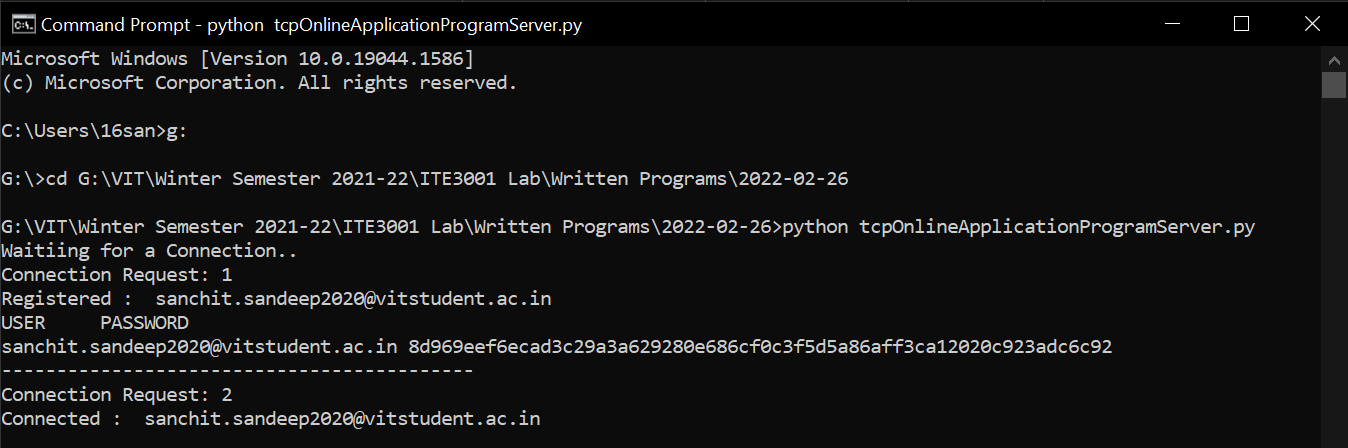
\includegraphics[width=\textwidth]{tcpOnlineApplicationProgramServer.png}
\caption{Server output}
\end{figure}
\begin{figure}[h] % h - Place the float here, i.e., approximately at the same point it occurs in the source text (however, not exactly at the spot)
\centering
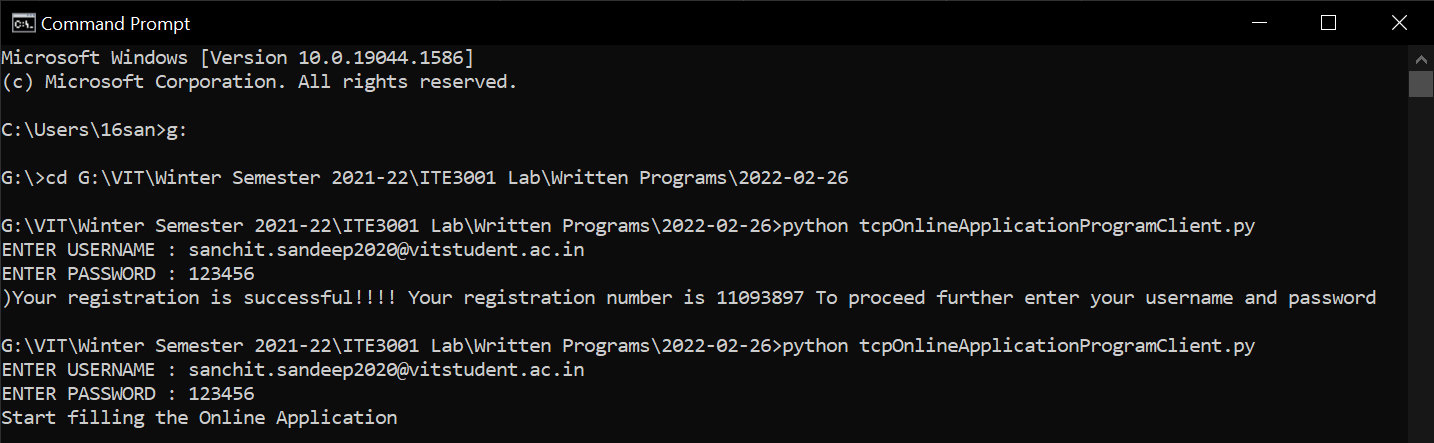
\includegraphics[width=\textwidth]{tcpOnlineApplicationProgramClient.png}
\caption{Client output}
\end{figure}
\newpage

Q2. Implement a UDP socket based ATM System. Make the server to maintain the customer details (name, card no, pin and balance). When a client wants to withdraw amount, validate his login with card no & pin, display a welcome message and perform the withdraw operation if he is having sufficient balance or display a warning message.. \newline
Ans- \\ Code- \\ udpATMServer.py-\inputminted{python}{udpATMServer.py}
udpATMClient.py- \inputminted{python}{udpATMClient.py}
Output-
\begin{figure}[h] % h - Place the float here, i.e., approximately at the same point it occurs in the source text (however, not exactly at the spot)
\centering
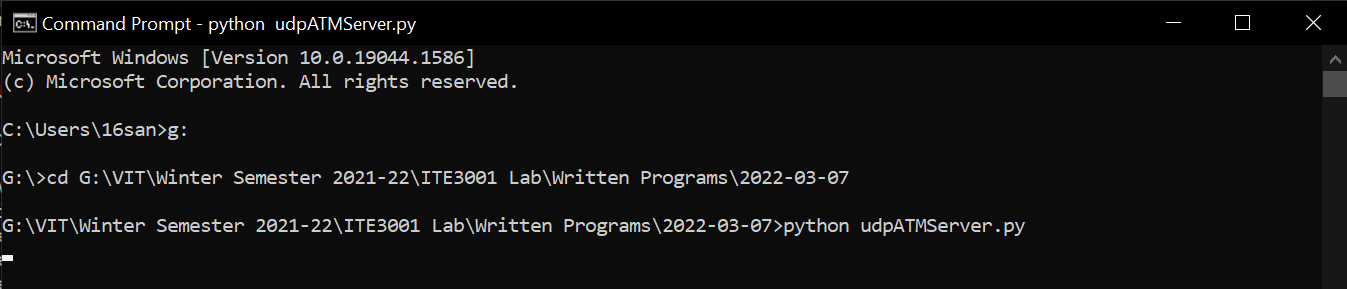
\includegraphics[width=\textwidth]{udpATMServer.png}
\caption{Server output}
\end{figure}
\begin{figure}[h] % h - Place the float here, i.e., approximately at the same point it occurs in the source text (however, not exactly at the spot)
\centering
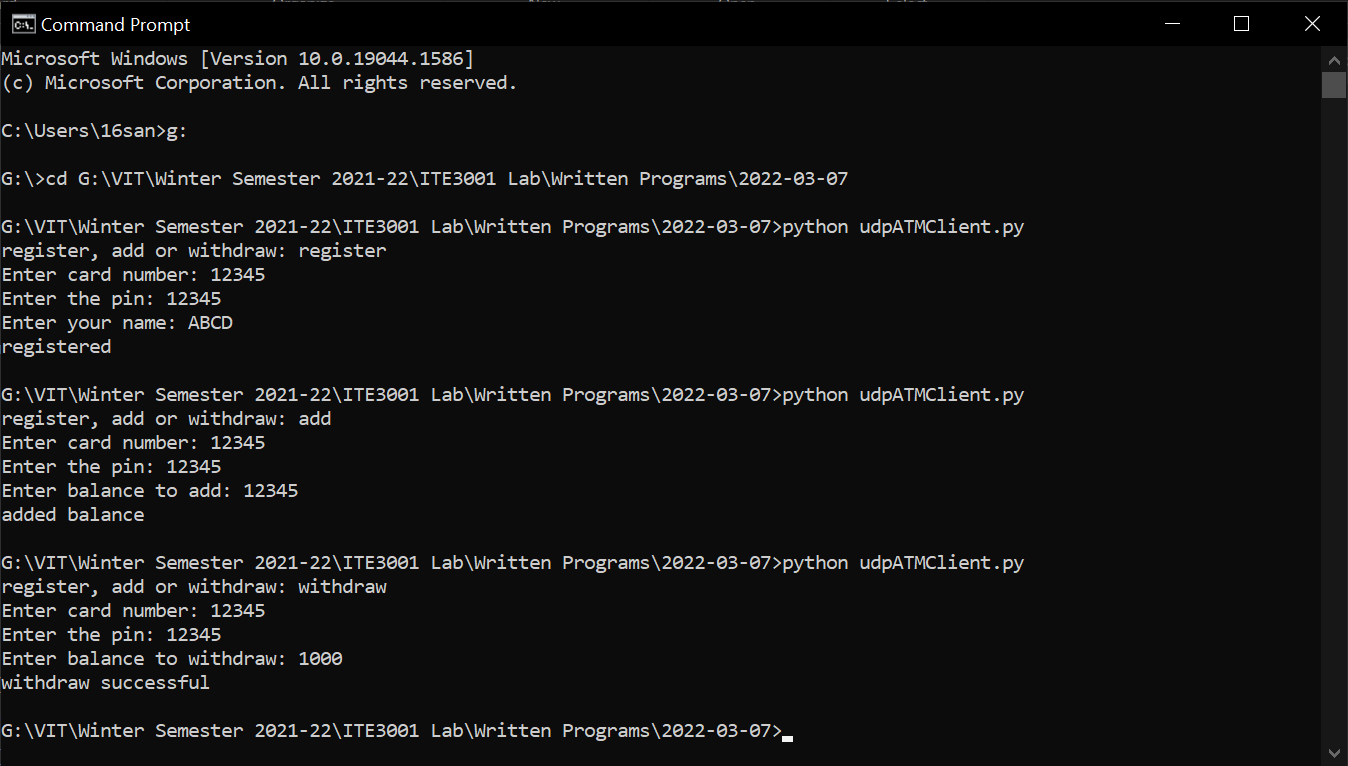
\includegraphics[width=\textwidth]{udpATMClient.png}
\caption{Client output}
\end{figure}
\newpage
Q3. Develop a UDP client/server application for transferring contents of a text file from client to server.
Ans- \\ Code - \\ udpFileServer.py-\inputminted{python}{udpFileServer.py}
udpFileClient.py- \inputminted{python}{udpFileClient.py}
\newpage
Output-
\begin{figure}[h] % h - Place the float here, i.e., approximately at the same point it occurs in the source text (however, not exactly at the spot)
\centering
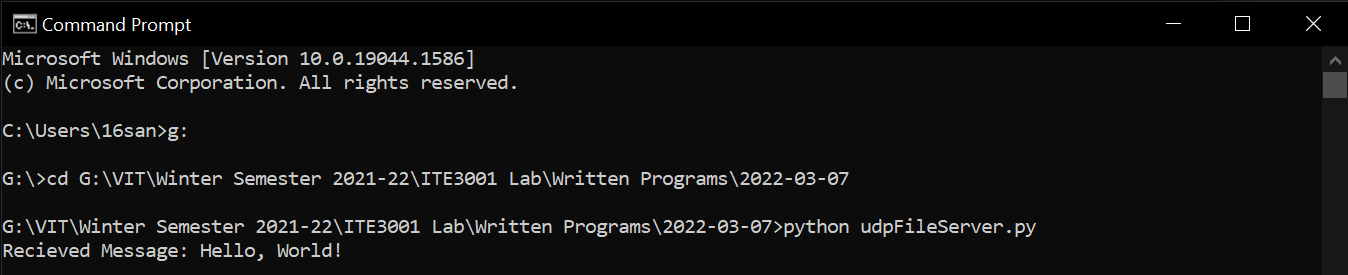
\includegraphics[width=\textwidth]{udpFileServer.png}
\caption{Server output}
\end{figure}
\begin{figure}[h] % h - Place the float here, i.e., approximately at the same point it occurs in the source text (however, not exactly at the spot)
\centering
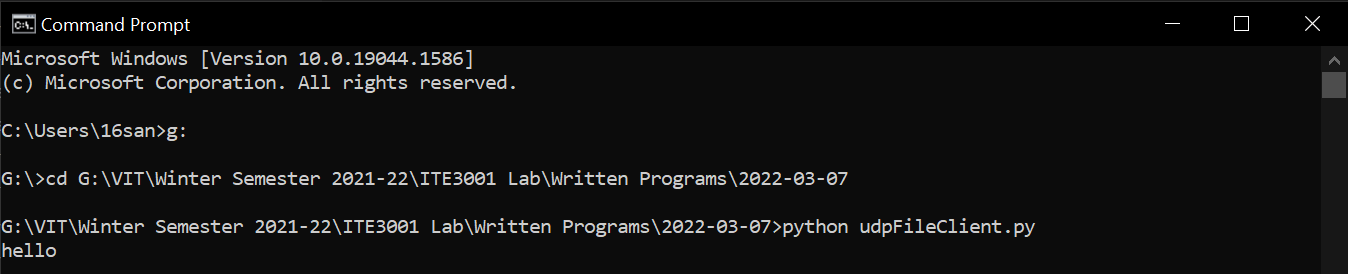
\includegraphics[width=\textwidth]{udpFileClient.png}
\caption{Client output}
\end{figure}
\newpage
Q3.Write a UDP based client-server program to calculate the age from the date of birth of the client as on today. Client has to send first name, last name, year, month and day of birth to the server. The server will first concatenate the two names to get the client name and then it will calculate the age. For example, if the date of birth of a user is 1/07/2001 then his age is 14 years 0 months and 17 days if today's date is 18/07/2015. Get today's date from the server. Server will send a message to the client that “(Client Name) Your age is ----years--months --days”.
Ans- \\ Code - \\ udpDOBServer.py-\inputminted{python}{udpDOBServer.py}
udpDOBClient.py- \inputminted{python}{udpDOBClient.py}
Output-
\begin{figure}[h] % h - Place the float here, i.e., approximately at the same point it occurs in the source text (however, not exactly at the spot)
\centering
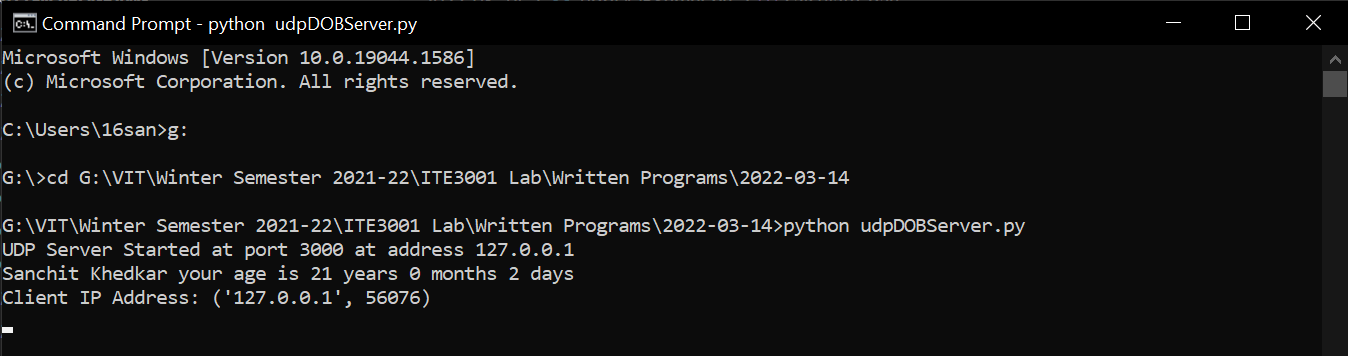
\includegraphics[width=\textwidth]{udpDOBServer.png}
\caption{Server output}
\end{figure}
\begin{figure}[h] % h - Place the float here, i.e., approximately at the same point it occurs in the source text (however, not exactly at the spot)
\centering
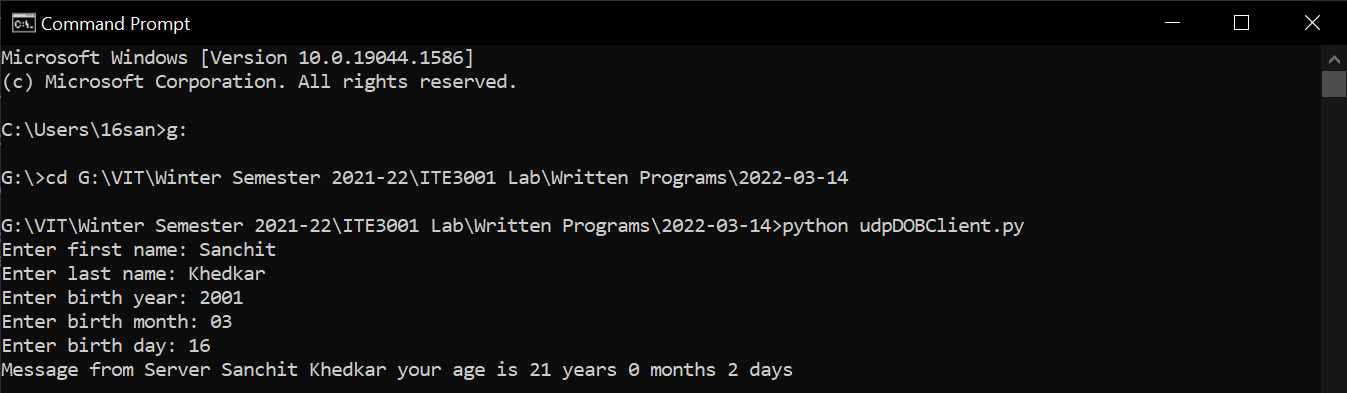
\includegraphics[width=\textwidth]{udpDOBClient.png}
\caption{Client output}
\end{figure}
\end{document}
